\documentclass[a4paper,10pt]{article}
\usepackage[english]{babel}
\usepackage[utf8]{inputenc}
\usepackage{url}
\usepackage[margin=1in]{geometry}
\usepackage{enumitem}

\usepackage[nottoc]{tocbibind}
\usepackage{fancyvrb} 
\usepackage{float}
\usepackage{graphicx}
\usepackage{subcaption}
\usepackage{color}
\usepackage{booktabs}
\usepackage{listings}

\title{Combinatorial Optimization\\Homework 5 – 3SAT Genetic Algorithm}
\author{Matyáš Skalický\\skalimat@fit.cvut.cz}

\begin{document}
\maketitle
\tableofcontents
\medskip

\section{Experiment Setting}
The problem of finding a solution to the boolean formula is called boolean satisfiability problem (SAT). In this homework, we are trying so solve a special class of SAT called \emph{Weighted 3SAT}. In 3SAT, the boolean problem is presented in a conjunctive normal form where all clauses contain exactly three literals. Since the problem is weighted, we are trying to come up with a solution that satisfies the boolean formula while maximizing the sum of weights for the literals that are assigned as true.

To make the measurements fair across different population sizes (further, we also call the population a batch), each experiment is ran for \emph{$2$ seconds} of the CPU time. It is possible that for some settings, the SAT problem isn't solved in this time.

The homework was programmed in Python. To speed-up the computation, as many computations as possible were implemented as vectorized numpy operation. Also, the experiments were ran in parallel on a server with $40$ cores to make the experiments feasible.

\section{Genetic Algorithm}

The implemented genetic algorithm solver is parametrized mainly by 4 hyperparameters:

\begin{description}
	\item[Mutation Rate]{Probability of randomly flipping a literal's value.}
	\item[Batch Size]{Size of the population.}
	\item[Init Type]{How each individual is initialized.}
	\item[Fitness Type]{Which fitness function is used.}
\end{description}

Generally speaking, we first randomly spawn a pool of instances. Before the CPU time runs out, we repeatedly take a batch of parent instances, and by using selection, recombination and mutation, we create a pool of children of the same size. The detailed steps are described below.

\subsection{Fitness}

Fitness should ideally copy the value of the function which we want to optimize. In case of weighted 3SAT, we are working with 2 objectives which we want to accomplish:

\begin{itemize}
	\item Find a binary assignment that solves the boolean formula.
	\item Maximize the weights of the selected literals.
\end{itemize}

Solving 3SAT is very different from solving the knapsack problem. In knapsack problem, it is trivial to find a feasible solution. Most of the work is then done in optimizing the contents of the bag. In 3SAT, finding any feasible instance is contrary to the knapsack problem very hard. Finding the instance with the highest sum of literal weights further increases the complexity of finding the solution.

In a sense, we operate in 2 modes. In the first mode, we don't know any solution to the 3SAT problem. In the second mode, we have found the solution, but we need to improve the assignment of the literals in order to maximize the weights.

Figuring out the fitness score in genetic algorithms is one of the hardest tasks. First, how do we \emph{push} the algorithm towards solving the SAT problem? And then, how do we design the fitness score in order to keep improving? I have designed two experimental fitness score methods:

\begin{description}
	\item[sum or nothing] Fitness score is $0$ if the solution isn't feasible. Otherwise, it represents the sum of the literals which are assigned true.
	\item[correct count] If current assignment solves the problem, use the sum of weights of the true literals. If it isn't solved, count how many clauses are correctly solved. This helps early on, when no solution was found.
\end{description}

\subsection{Random Initialization}

I've implemented 2 initialization strategies for instance intialization. The \emph{all false} strategy initialized all literals as false. The \emph{uniform} strategy randomly selects how each literal is initialized.

\subsection{Selection}

Selection takes a pool (batch) of candidates on the input. It calculates the total fitness and uses the roulette wheel selection to find the pairs of candidates that go into recombination.

\subsection{Recombination}

We take 2 input instances (\emph{parents}). A single-point crossover is used to create 2 children. If any of the children is valid (fitness is non-0), we return the better child. Otherwise, the better parent is returned.

\subsection{Mutation}

Mutation is controlled by the \emph{mutation\_rate} hyperparameter. It is called on the instances that come out of recombination before we add them into children pool. We randomly flip the value assigned to the literal with the probability defined by the \emph{mutation\_rate}.

\section{Experiments}

As described above, we are running each experiment for $2$ seconds of the CPU time to make different batch sizes comparable. Small batches will be much faster, but there will be less diversity in the population. Large batches will contain diverse initialization pools (depending on the init strategy), but the processing will be much slower.

\subsection{Pilot Experiments}

During the pilot experiments, we would like to determine the ideal combination of hyperparameters (batch size, mutation rate, initialization strategy and fitness function) to solve the weighted 3SAT problem. We will start with smaller instances of \lstinline{wuf20-78} in order to make the pilot experiments a bit faster.



\begin{figure}[!htb]
	\centering
  	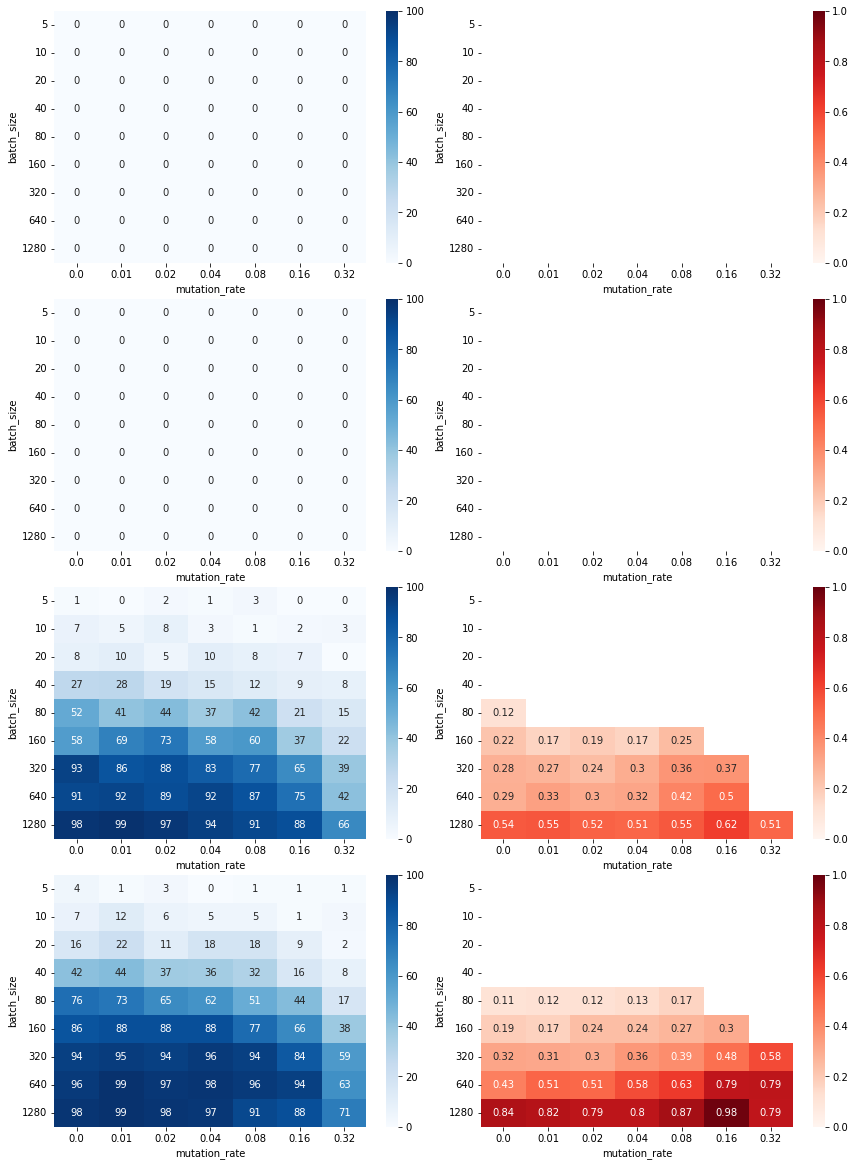
\includegraphics[width=\textwidth]{images/pilot_counts_means.png}
	\caption{Random Initialization; 3s Runtime; Instance Size 40}
	\label{detail}
\end{figure}

As described before, the naive initialization produces very sparse bags. With very low mutation rate, there isn't enough diversity in the initial population pool to achieve good performance. As we can see in the Figure \ref{pilot_naive}, a small mutation rate is required. Interesting finding is that we are able to solve the problem even with a very small batch size. Even though the batch size is very small, the algorithm will be very fast. And it is able to go through many iterations before the time runs out.

The random initialization contains fuller bags which contain a larger number of items. Figure \ref{pilot_random} shows, that even if the mutation rate is $0$, the algorithm achieves good results given large batch size. 

\subsection{Detailed Experiment}

The random initialization strategy has worked slightly better than the naive strategy. The best set of hyperarameters would be batch size of $320$ and mutation rate of $0.02$ (2\%). We will now look in a finer detail at the fitness score over time for the best obtained hyperparameter combination.

As we can see in the Figure \ref{detail}, for the instance above, the ideal solution was found just after $1$ second. Yet, we can see that the mean relative bag value across the population is still going up. It however levels after $2$ seconds.

\clearpage
\section{Discussion and Takeoffs}

Fourth homework was much more fun compared to the previous one. Genetic algorithms are one of my favorite black-box methods and even though I've implemented them several times, I still had fun applying it on the knapsack problem.

There was one interesting takeaway that came from the way I measured the experiment in the pilot phase (fixed amount of CPU time). The algorithm was able to find a good solution even with a very small population size of $5$ given that the mutation was turned on and was small. This is because the algorithm is able to go through a large amount of iterations before the time runs out as opposed to the large populations. But this relates to the NK algorithm and the knapsack problem itself.

\end{document}